
%%%%%%%%% MASTER -- compiles the sections

\documentclass[11pt,letterpaper]{article}
\setlength{\parskip}{1ex plus 0.5ex minus 0.2ex}

\usepackage{graphicx}
\usepackage{hyperref}
\hypersetup{
    colorlinks,%
    citecolor=black,%
    filecolor=black,%
    linkcolor=black,%
    urlcolor=black
}
\usepackage{listings} %for source code figures
\usepackage[toc,xindy,style=long3colheaderborder,footnote]{glossaries}
%\usepackage[toc,xindy]{glossaries}
\makeindex
\makeglossaries


\newglossaryentry{speedup}{name={speedup}, description={The overall time gain of a process or computation.}}

\newglossaryentry{time complexity}{name={time complexity}, description={The time it takes for a process to run.}}


\newglossaryentry{paralellization}{name={paralellization}, description={Taking independent or semi-independent processes, and processing them in parallel (at the same time).}}

\newglossaryentry{granularity}{name={granularity}, description={The time or portion of the process that each iteration / sub-process takes.}}

\newglossaryentry{HPC}{name={HPC}, description={High Performance Computing.}}


%%%%%%%%%%%%%%%%%%%%%%%%%%%%%%%%%%%%%%%%%%%%%%%%%%%%%%%%%%%%%%%%%%%%%%%%%
\pagestyle{plain}                                                      %%
%%%%%%%%%% EXACT 1in MARGINS %%%%%%%                                   %%
\setlength{\textwidth}{6.5in}     %%                                   %%
\setlength{\oddsidemargin}{0in}   %% (It is recommended that you       %%
\setlength{\evensidemargin}{0in}  %%  not change these parameters,     %%
\setlength{\textheight}{8.5in}    %%  at the risk of having your       %%
\setlength{\topmargin}{0in}       %%  proposal dismissed on the basis  %%
\setlength{\headheight}{0in}      %%  of incorrect formatting!!!)      %%
\setlength{\headsep}{0in}         %%                                   %%
\setlength{\footskip}{.5in}       %%                                   %%
%%%%%%%%%%%%%%%%%%%%%%%%%%%%%%%%%%%%                                   %%
\newcommand{\required}[1]{\section*{\hfil #1\hfil}}                    %%
\renewcommand{\refname}{\hfil References Cited\hfil}                   %%
\bibliographystyle{plain}                                              %%
%%%%%%%%%%%%%%%%%%%%%%%%%%%%%%%%%%%%%%%%%%%%%%%%%%%%%%%%%%%%%%%%%%%%%%%%%

%PUT YOUR MACROS HERE

\date{Spring 2012}
\title{Team EcoData - Hatch Tool\\
}

\author{Mike Solomon\\
	Colby Blair \\
	Computer Science Undergraduates \\
	University of Idaho Computer Science Department\\
	CS 481 Capstone Project \\
}


\begin{document}

\section*{Letter of Transmittal}
\textbf{Subject.} High Performance Computing in Natural Resources.

\textbf{Purpose.} This report focuses on Hatch project, and the challenges with managing data in the
scientific research environment. The goal is to introduce new approaches to organizing data, and making
it more searchable. The Hatch project creates a foundation for a tool that allows users to upload, search,
format, and visualize their data in ways they didn't think of before. This report highlights some of the 
problems with computation and data management in the current research environment, and makes 
suggestions for new approaches. It talks about specific algorithms for searching data, and standards for
formatting and storing it.

\textbf{Background.} The amount of data being stored in scientific databases today is growing 
exponentially. The amount of computational power in cpu's, however, is no longer growing exponentially.
The consequence is an gap opening between data and results. Researchers are trying to build and rebuild
their computational infrastructure, to try to get computational growth back to the pace of data growth.
But in this report, we suggest a complimentary approach to computing research data. The Hatch project
comes from the idea that a significant amount of research data is redundant or not wanted. But it is also
vast and not managable. Researchers end up wasting computation time on data points and sets that they do 
not care about, at the expense of ones they do care about.

\textbf{Preliminary Work}. With the experience of the authors of this report, there is more than 8 years of work in computer science, bioinformatics, and natural resources. There is 2+ years of work in computing
clusters for the University of Idaho Initiative for Bioinformatics and Evolutionary STudies (IBEST), as well as 
1.5 years of research in wildlife management. 

\thispagestyle{empty}

\pagebreak

\maketitle

\thispagestyle{empty}

\pagebreak

\thispagestyle{empty}
\tableofcontents
\listoffigures

\pagebreak

\begin{abstract}
With today's exponential increase of data, the demand for processing is outpacing the supply. The way we 
processed data yesterday would take years to do today. Unfortunately, the lack of fluency with computing in
today's research proposals results in processing a fraction of the data collected. This weakens research 
projects, and leads to a lot of unnecessary data collection. 

Today's researchers need tools to become more efficient with processing data. Until computation can keep
up again with exponential data growth, researchers will need to carefully select the data that they want to 
do research on, and throw away data that will not yield results. The users of such tools range anywhere from
fish researchers in the Columbia Basin, to bioinformaticians, to economists, and more. Having more 
searchable, usable data applies to almost everyone, and the use cases and usefulness of a tool like Hatch
are endless.

\end{abstract}

\setcounter{page}{1}

\pagebreak

%
%%%%%%%%% SUMMARY -- 1 page, third person
% e.g:  "The PI will prove" not "I will prove"

%Introduction / Summary (1 page).  The following information is typically included in proposal introductions for this 
%grant. The summary should lead to the proposal body but it should also be a self-contained document, 
%summarizing what is being proposed and why.   
 
% Provide appropriate background that sets the context for the problem and the objectives. 
%State the specific problem (may also be thought of as a need, central research question, or hypothesis) 
%your research will address. 
% State the objectives of the proposed research. 
%State any limits of the proposed research  (may not be needed). 
%Summarize the research methods you will use to achieve research objectives (if clearly covered elsewhere 
%in the introduction, a separate section may not be needed). 


%\required{Project Summary}
\section{Project Summary}
% This should be a brief statement of the problem you plan to address.
% It should look something like an abstract. 
In today's scientific environment, there is a growing focus on data storage and
processing. Some of the largest problems scientists face are related to the data
deluge, and the inability to conceptalize problem and solutions from large
tracts of data. The result is many attempts by scientific professionals to 
design software, leading to many bad software designs. Vast amounts of 
expensively collected data never get processed, 
because the software designs take so much maintenance. Data is often duplicated,
often in different locations, lost, or never makes it from collection to 
analysis. The overall lack of system designs to handle the data further 
hinders analysis.

This proposal is for a project that helps solve these design problems for 
many scientists. The project is a data harvester and organizer tool. It
is a local web interface that allows scientists to collect, query, organize, 
and share data with other researchers.
Many of these scientists work with similar data sets, ask different 
questions, and need immediate search tools. The proposed tool would first allow 
users to visualize and filter data, and secondly prepare and ship the data
off for analysis. It also helps users visualize data graphically, to 
help the conceptualize, organize, and refine data, before transporting and 
processing it. This 
project proposes using PTAG and othe ecological data sets from the Columbia 
Basin to test design, but should be exdendable to many different users with very
different data sets.

The tool will not overlap with the functionality of existing tools like 
PTAGIS or DART. It will carefully handle data sharing,
choosing opt-in, lock-down policies by default.

\subsection{Background}
%this section needs more stats and citations
In the Columbia Basin today, millions of federal dollars are spent on PTAG 
and othe systems to collect environmental data. 
This data includes fish location, ecological community composition, and 
abiotic data. Yet, the project 
results from most research are far from concrete. Despite the lack of 
understandable results, important decisions that affect the local environment 
and economy have to be made. Decisions like whether or not to conduct 
major habitat restoration projects. 

%We should cite something other study / examples in the basin. Foster's talk
% just sticks in my head as a good example
The Columbia Basin is just one small example. Bioinformatics is another 
data intesive study that generates more data that it can process. Its 
%is this 10%? It may be lower
estimated that less than 10\% of the data collected by bioinformatic 
researchers at the University of Idaho actually makes it through proccessing
\cite{foster}. The rest has to be filtered as best as can be managed, and the 
low value data trimmed out. The problem with 10\% data use, is that not just 
the fat, but the meat and bone has to be cut away. Either significantly more
data must be analyzed, or significantly less should be collected. At the very
least, storing the data in an easily readable format can show where the 
gaps are. So far, our experience and research shows similar shortfalls in 
data analysis in the Columbia Basin.

\subsection{Problem Statement}
One of the biggest problems researchers in the Columbia Basin have is getting
their data somewhere meaningful. Central databases like PTAGIS offer a 
central storage and clients can push data there, but they don't offer useful
tools for managing data. Once the data is pushed, it is hard to access and
manipulate. 
%stuff to massage
% I hate to get rid of the next bit, because it is some of the buzz that the
% project approvers are looking for. Can we work this verbage in without it
% being a priority / main focus?
Researchers are often in remote locations, and have low bandwidth
connections. 
% end stuff to massage
Creating a robust tool will guarantee ease of use for the data, no matter
the location.

Many researchers have significant data management tasks before even thinking 
about pushing data to the cloud. Once they are ready, they need seemless ways to
synchronize data to and from the cloud. They also may want to query their data,
and filter it into small subsets. Most researchers don't have time to learn
new programming language or interfaces. They need a data management tool 
that has a user 
interface that is familiar to use cases they already understand. Once they
have created a data subset, they will want to share it, save it, copy it, 
and compare it with other data sets. Getting the right data to the right place 
in the right amount of time is crucial.

\subsection{Objectives}

\begin{figure}[!h]
        \begin{center}
		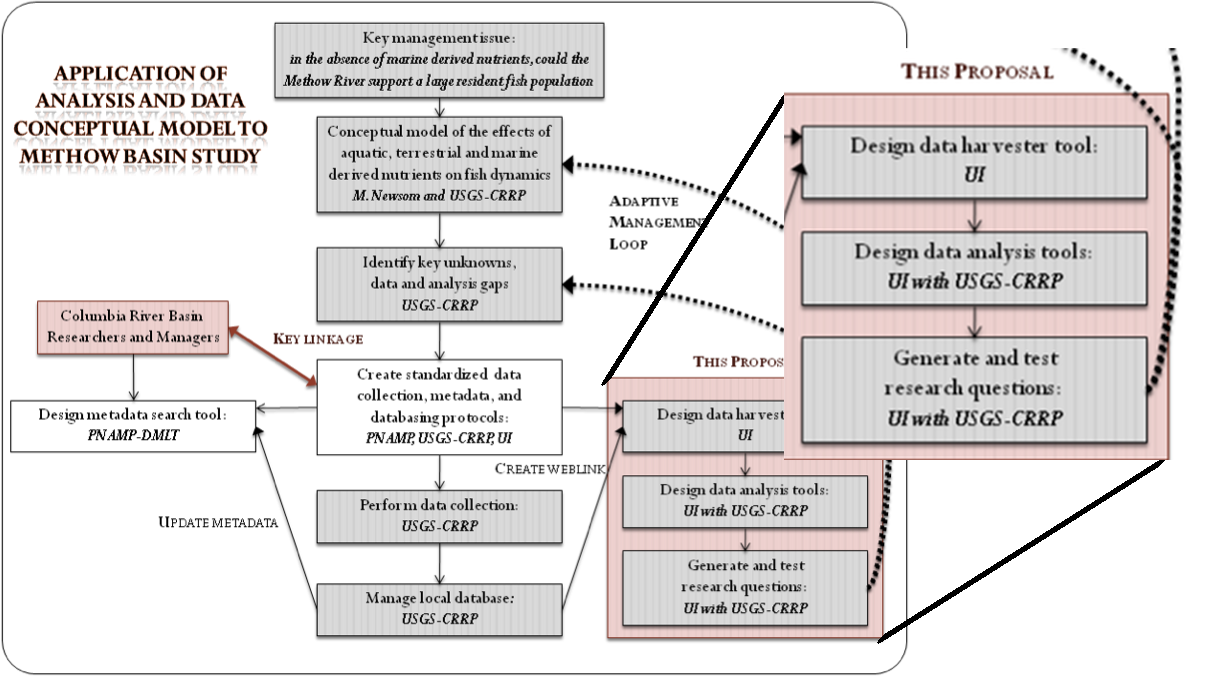
\includegraphics[width=120mm]{images/combo_proposal}
                \caption{This proposal software's application domain in DE-CRRP}
                \label{combo_proposal}
        \end{center}
\end{figure}

The proposed project will tackle the UI data harvester portion of the grant 
funded USGS-CRRP project (Figure \ref{combo_proposal}), directed by Alex 
Fremier of the UI College of Natural Resources. The data management tool
will be a web-like GUI that can be installed locally on the clients' computers.
The tool will contain a expandable meta data server 
that can be connected to others, for a \textbf{decentralized} data storage
cloud. The cloud will consist of the many instances of the tool, acting as a
cloud of 
\textbf{decentralized databases}. It will contain an interface to an existing 
or custom \textbf{networking protocol} that will allow for many different data 
formats to be synchronized across the cloud. The project will also have graphic
interfaces for \textbf{seamless data management}.

The decentralized cloud model allows some serious advantages to researchers.
They can see exactly what their data looks like, before they submit it.
They can filter out bad data before it consumes bandwidth, and can retract
undesirable data from the cloud, even after synchronizing it. It also frees
them from central storage service management and fees, and 
\textbf{encourages internode and inter-research communication}. 
The tool can be setup
on multiple hosts, and can be used for the benefits of 
the centralized cloud model. Each client can decide what topology suites them 
best.

The decentralized cloud model implements a distributed database model.
Distributed databases increase availability and reliability. They are more
easily expandable, and can better protect from data loss from local disasters or
malicious attacks. Moving data to where it is in highest demand also increases
query performance. Offloading archive data to remote site with more 
resources preserves local resources. Replicated datasets can guarantee 
better availability. By staging data locally and filtering it before allowing
it to be exchanged, the autonomy of the organization is better preserved. 

%probably some specific network protocols, like SOAP, etc, should be mentioned
%Alex, the network protocol doesn't have to apply just to low bandwidth users
%, but also to large data transfers
The network protocol will allow incremental synchronization of data from host
to host, even in less reliable environments. The tool will create
an \textbf{outreach} from researchers in high availability areas to those
in low availability, low bandwidth areas, and back. The network protocol
will have support for major data formats (i.e. SQL, CSV, more), and allow
users to send incremental pieces of the data. In the case of very large 
data sets or low bandwidth, the receiver of the data can still use it. Whether 
the data takes more time to transfer, or never completes.

The seamless interface will allow users to sort their data needing only 
basic knowledge of computers. Users will be able their mouse to select
datasets and apply filters to them. The tool will allow them to query local or
remote data, or to dynamically join both. Queries will create data subsets that
users can bring to a workspace. The tool will be able to sort data however
the user likes, on the fly. It will then be able to graph the ranges in 
the subset in most ways the user could want to sort them.

Once the user has manipulated their data subset to their satisfaction, they
will be able to save it in the meta data server's format, or in a set of major
data formats. The tool will also have analysis modules that will allow them
to run analysis on the local host. These modules will be extensible to running 
analysis jobs on other designated compute hosts, like workstations, clusters,
or even Amazon's EC2. The tool will come only with basic functionality for 
local analysis modules, but will be extensible to the heavier compute options.
%\required{Intellectual Merit}
% This is why your project is interesting and will help further
% knowledge in the field of mathematics. 

%\required{Broader Impacts}
% There are 4 kinds of broader impacts.
% 1. advance discovery and understanding while promoting teaching,
% training and learning
% 2. broaden the participation of underrepresented groups
% 3. disseminated broadly to enhance scientific and technological
% understanding
% 4. benefits of the proposed activity to society

 % - this stuff is ok, but I think the proposal stuff is better

%%%%%%%%% SUMMARY -- 1 page, third person
% e.g:  "The PI will prove" not "I will prove"

%Introduction / Summary (1 page).  The following information is typically included in proposal introductions for this 
%grant. The summary should lead to the proposal body but it should also be a self-contained document, 
%summarizing what is being proposed and why.   
 
% Provide appropriate background that sets the context for the problem and the objectives. 
%State the specific problem (may also be thought of as a need, central research question, or hypothesis) 
%your research will address. 
% State the objectives of the proposed research. 
%State any limits of the proposed research  (may not be needed). 
%Summarize the research methods you will use to achieve research objectives (if clearly covered elsewhere 
%in the introduction, a separate section may not be needed). 


%\required{Project Summary}
\section{Project Summary}
% This should be a brief statement of the problem you plan to address.
% It should look something like an abstract. 
In today's scientific environment, there is a growing focus on data storage and
processing. Some of the largest problems scientists face are related to the data
deluge, and the inability to conceptalize problem and solutions from large
tracts of data. The result is many attempts by scientific professionals to 
design software, leading to many bad software designs. Vast amounts of 
expensively collected data never get processed, 
because the software designs take so much maintenance. Data is often duplicated,
often in different locations, lost, or never makes it from collection to 
analysis. The overall lack of system designs to handle the data further 
hinders analysis.

This proposal is for a project that helps solve these design problems for 
many scientists. The project is a data harvester and organizer tool. It
is a local web interface that allows scientists to collect, query, organize, 
and share data with other researchers.
Many of these scientists work with similar data sets, ask different 
questions, and need immediate search tools. The proposed tool would first allow 
users to visualize and filter data, and secondly prepare and ship the data
off for analysis. It also helps users visualize data graphically, to 
help the conceptualize, organize, and refine data, before transporting and 
processing it. This 
project proposes using PTAG and othe ecological data sets from the Columbia 
Basin to test design, but should be exdendable to many different users with very
different data sets.

The tool will not overlap with the functionality of existing tools like 
PTAGIS or DART. It will carefully handle data sharing,
choosing opt-in, lock-down policies by default.

\subsection{Background}
%this section needs more stats and citations
In the Columbia Basin today, millions of federal dollars are spent on PTAG 
and othe systems to collect environmental data. 
This data includes fish location, ecological community composition, and 
abiotic data. Yet, the project 
results from most research are far from concrete. Despite the lack of 
understandable results, important decisions that affect the local environment 
and economy have to be made. Decisions like whether or not to conduct 
major habitat restoration projects. 

%We should cite something other study / examples in the basin. Foster's talk
% just sticks in my head as a good example
The Columbia Basin is just one small example. Bioinformatics is another 
data intesive study that generates more data that it can process. Its 
%is this 10%? It may be lower
estimated that less than 10\% of the data collected by bioinformatic 
researchers at the University of Idaho actually makes it through proccessing
\cite{foster}. The rest has to be filtered as best as can be managed, and the 
low value data trimmed out. The problem with 10\% data use, is that not just 
the fat, but the meat and bone has to be cut away. Either significantly more
data must be analyzed, or significantly less should be collected. At the very
least, storing the data in an easily readable format can show where the 
gaps are. So far, our experience and research shows similar shortfalls in 
data analysis in the Columbia Basin.

\subsection{Problem Statement}
One of the biggest problems researchers in the Columbia Basin have is getting
their data somewhere meaningful. Central databases like PTAGIS offer a 
central storage and clients can push data there, but they don't offer useful
tools for managing data. Once the data is pushed, it is hard to access and
manipulate. 
%stuff to massage
% I hate to get rid of the next bit, because it is some of the buzz that the
% project approvers are looking for. Can we work this verbage in without it
% being a priority / main focus?
Researchers are often in remote locations, and have low bandwidth
connections. 
% end stuff to massage
Creating a robust tool will guarantee ease of use for the data, no matter
the location.

Many researchers have significant data management tasks before even thinking 
about pushing data to the cloud. Once they are ready, they need seemless ways to
synchronize data to and from the cloud. They also may want to query their data,
and filter it into small subsets. Most researchers don't have time to learn
new programming language or interfaces. They need a data management tool 
that has a user 
interface that is familiar to use cases they already understand. Once they
have created a data subset, they will want to share it, save it, copy it, 
and compare it with other data sets. Getting the right data to the right place 
in the right amount of time is crucial.

\subsection{Objectives}

\begin{figure}[!h]
        \begin{center}
		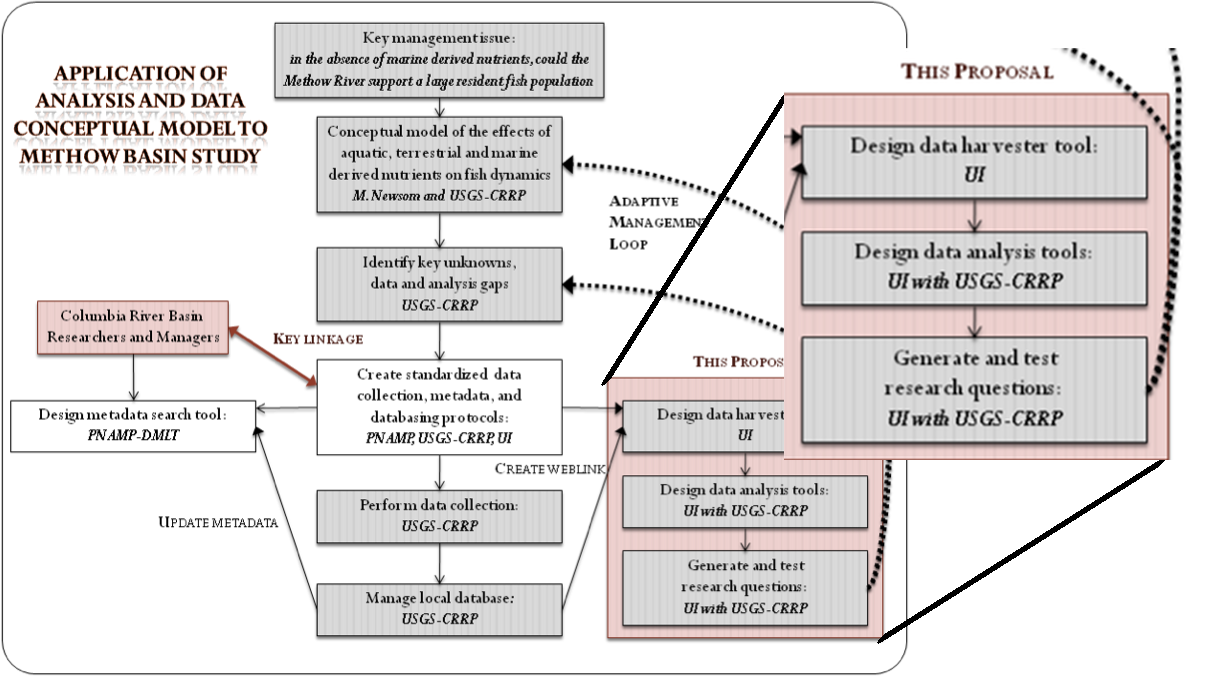
\includegraphics[width=120mm]{images/combo_proposal}
                \caption{This proposal software's application domain in DE-CRRP}
                \label{combo_proposal}
        \end{center}
\end{figure}

The proposed project will tackle the UI data harvester portion of the grant 
funded USGS-CRRP project (Figure \ref{combo_proposal}), directed by Alex 
Fremier of the UI College of Natural Resources. The data management tool
will be a web-like GUI that can be installed locally on the clients' computers.
The tool will contain a expandable meta data server 
that can be connected to others, for a \textbf{decentralized} data storage
cloud. The cloud will consist of the many instances of the tool, acting as a
cloud of 
\textbf{decentralized databases}. It will contain an interface to an existing 
or custom \textbf{networking protocol} that will allow for many different data 
formats to be synchronized across the cloud. The project will also have graphic
interfaces for \textbf{seamless data management}.

The decentralized cloud model allows some serious advantages to researchers.
They can see exactly what their data looks like, before they submit it.
They can filter out bad data before it consumes bandwidth, and can retract
undesirable data from the cloud, even after synchronizing it. It also frees
them from central storage service management and fees, and 
\textbf{encourages internode and inter-research communication}. 
The tool can be setup
on multiple hosts, and can be used for the benefits of 
the centralized cloud model. Each client can decide what topology suites them 
best.

The decentralized cloud model implements a distributed database model.
Distributed databases increase availability and reliability. They are more
easily expandable, and can better protect from data loss from local disasters or
malicious attacks. Moving data to where it is in highest demand also increases
query performance. Offloading archive data to remote site with more 
resources preserves local resources. Replicated datasets can guarantee 
better availability. By staging data locally and filtering it before allowing
it to be exchanged, the autonomy of the organization is better preserved. 

%probably some specific network protocols, like SOAP, etc, should be mentioned
%Alex, the network protocol doesn't have to apply just to low bandwidth users
%, but also to large data transfers
The network protocol will allow incremental synchronization of data from host
to host, even in less reliable environments. The tool will create
an \textbf{outreach} from researchers in high availability areas to those
in low availability, low bandwidth areas, and back. The network protocol
will have support for major data formats (i.e. SQL, CSV, more), and allow
users to send incremental pieces of the data. In the case of very large 
data sets or low bandwidth, the receiver of the data can still use it. Whether 
the data takes more time to transfer, or never completes.

The seamless interface will allow users to sort their data needing only 
basic knowledge of computers. Users will be able their mouse to select
datasets and apply filters to them. The tool will allow them to query local or
remote data, or to dynamically join both. Queries will create data subsets that
users can bring to a workspace. The tool will be able to sort data however
the user likes, on the fly. It will then be able to graph the ranges in 
the subset in most ways the user could want to sort them.

Once the user has manipulated their data subset to their satisfaction, they
will be able to save it in the meta data server's format, or in a set of major
data formats. The tool will also have analysis modules that will allow them
to run analysis on the local host. These modules will be extensible to running 
analysis jobs on other designated compute hosts, like workstations, clusters,
or even Amazon's EC2. The tool will come only with basic functionality for 
local analysis modules, but will be extensible to the heavier compute options.
%\required{Intellectual Merit}
% This is why your project is interesting and will help further
% knowledge in the field of mathematics. 

%\required{Broader Impacts}
% There are 4 kinds of broader impacts.
% 1. advance discovery and understanding while promoting teaching,
% training and learning
% 2. broaden the participation of underrepresented groups
% 3. disseminated broadly to enhance scientific and technological
% understanding
% 4. benefits of the proposed activity to society


\section{Database}

\subsection{Introduction}
One of the biggest challenges with Hatch was how to organize data. Specifically, pretty
much every organization with scientific data has their own standard or format on 
how they store research data. Many of these organizations want to share data between 
each other, but they cannot decide how to merge the formats. Consider the following
examples:

\begin{figure}[h]
	\begin{center}
	\begin{tabular}{ | c | c | c | }
		\hline
		site	&	datetime		&	unique fish tag	\\
		\hline
		TUC	&	02/16/06 19:08:15 	&	3D9.1BF1E7919A 	\\
		TUC	&	02/16/06 19:18:36 	&	3D9.1BF1A998FA 	\\
		TUC	&	02/17/06 18:21:03 	&	3D9.1BF20E8FE2	\\
		...	&	...			&	...		\\
		\hline
	\end{tabular}
	\caption{A database representing for PTAGIS data} 
	\label{ptagis_ex1}
	\end{center}
\end{figure}

\begin{figure}[h]
	\begin{center}
	\begin{tabular}{ | c | c | }
		\hline
		unique fish tag	&	DNA sequence	\\
		\hline
		3D9.1BF1E7919A 	&	ATGCTTAC...	\\
		3D9.1BF1A998FA 	&	TTACGATC...	\\
		3D9.1BF20E8FE2	&	GTGGASCT...	\\
		...		&	...		\\
		\hline
	\end{tabular}
	\caption{A database representation for DNA data} 
	\label{dna_ex1}
	\end{center}
\end{figure}

In each of the examples above, the data is represented with \textbf{rows} and 
\textbf{columns}, much the same way someone would represent the data in a Microsoft
Excel spreadsheet. These structures in a typical \textbf{relational database} (SQL, etc).
are called \textbf{tables}.

The above examples are simplifications of the rows and columns in actual research 
data. But they highlight one of the biggest issues with data storage using relational
databases: they require you to know the column names ahead of time. Not only that,
but they require that you know the data types of the values that go in those columns,
and once a table is created expecting a certain format, it is hard to change.

The problem with needing to know the structure of research data before designing
databases, is that research data \textbf{is semi-structured}, at best. Once it does
represent some structure, it often changes. For example, once researchers finally 
decide what columns and data types should go in the table in Figure \ref{ptagis_ex1},
another researcher suggests more columns that should go in to the table.

This leads to endless edits to the database and program design by some software 
developer. The standard table format that everyone can agree on isn't useful to many
researchers, because it usually leaves out a lot of other needed columns and fields.

A better approach is needed. Researchers, not committees, should decide how to store 
data. Data should be mergable based on common values in different tables (like the 
\textbf{unique fish tag} column in Figures \ref{ptagis_ex1} and \ref{dna_ex1}. The 
person who inputs the data should decide how one particular dataset is stored in a 
database, and should be able to choose to store the same data in a different table 
format, how they choose. There should be a simple tool that helps them do this.

The following sections describe different approaches to implementing a database design
that enables data storage for dynamic or semi-structured data.


\subsection{Relation Databases with table creations}
This approach is the simplest and follows the concept of table creation for data sets
pretty closely. Basically, for each input document in the form of a spreadsheet, a new
SQL table is created. The columns names and type are determined from the headers and 
data values in the spreadsheet.

\begin{figure}[h]
	\begin{center}
	\begin{lstlisting}
		CREATE TABLE ptagis_doc1
			(
				id int, 
				site char(50), 
				read_data_time date,
				tag char(50)
			); 
	\end{lstlisting}
	\caption{The SQL syntax for creating the table in Figure \ref{ptagis_ex1} } 
	\label{ptagis_ex1_sql}
	\end{center}
\end{figure}

The biggest problem with this approach with this approach is that each document
in the database is a table. When searching for a specific document, the database 
typically searches for the table name. This search is linear, and with hundreds,
thousands, or hundreds of thousands of documents, frequently searching the database
to look for values would be infinitely slow and useless.

Another problem with this design, is that building an interface like a web gui would
be difficult and complicated. 


\subsection{Relational Databases with tables for each datatype}
Another approach is to create column tables for each data type, and let document 
tables just be collections of columns. Each of the document column values point to 
respective values in the column tables.

\begin{figure}[h]
	\begin{center}
	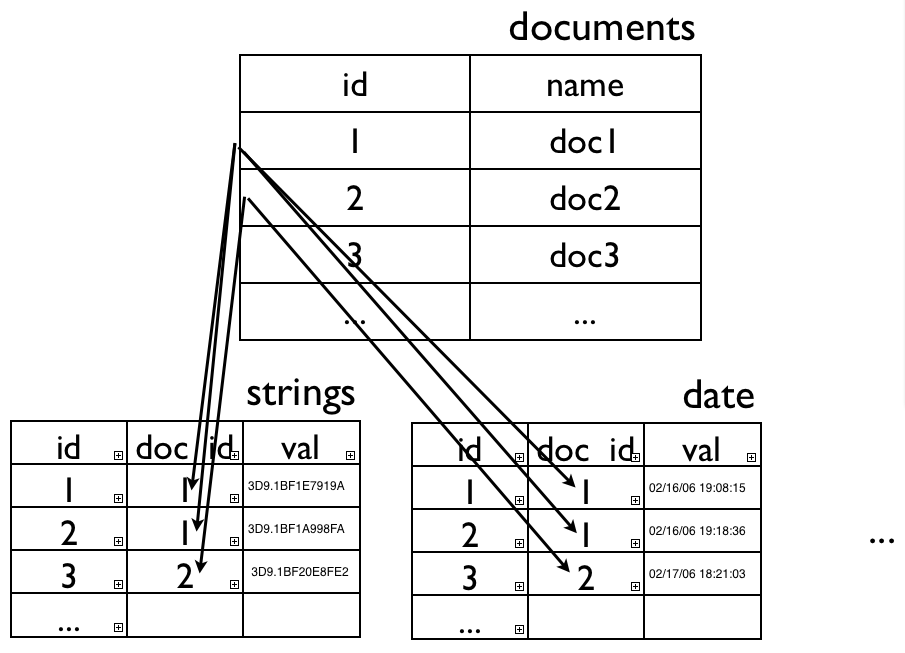
\includegraphics[width=80mm]{images/rel_db_lookup}
	\caption{Document table as a lookup table} 
	\label{rel_db_lookup}
	\end{center}
\end{figure}

This allows for documents to have a dynamic amount of columns with variable data types.
But there are two problems with this approach. First, for every value in every document
in the database, they are put into one table (i.e. all values with a 'string' data type
go into the 'string' table). With potentially millions of data values, each table
becomes an overflowing bucket, and don't utilize the the advantages of storing multiple
columns and values in one table. Searches for data would require lots of filtering 
for just the ones wanted for specific doucments, and would be inefficient.

The other issue is that every retrieval of data from a document would require lot and 
lots of lookups. Data retrieval over significantly high data sets would quickly become
very computationally intensive, and not practical.


\subsection{CouchDB}
When one thinks about the fundemental issues with storing, searching, and merging 
research data, a core issue is identified: data is semi-structured. This is what
makes trying to use relational databases so hard. They were made for datasets where
you knew the structure up front, and seldom wanted to change their structures.

The one assumption that Hatch makes about the data is that \textbf{there are rows and
columns}. This is the only assumption Hatch makes. This leaves the database and 
interface designs free from whatever changes are needed by the users.

This is done by storing data in JSON format. The data is stored in an array of hashes,
modeled exactly like how Ruby on Rails 3 returns records from its Active Record.
This allows users to input data however they like, define delimiters for columns using
Hatch Input Filters, and Hatch does the rest. It finds the most specific data type the
values can be stored in, skips non-matching entries, and populates all the forms on 
the web pages according to the data. All without actually knowing the structure of the 
data.

This leads to the technical implementation of the Hatch Database.


\subsection{Hatch Database}
Since Hatch uses Ruby on Rails, there are lots of tools and libraries for using the 
standard relational database, via Rails' Active Record. In many/most cases, Hatch
actually wants to stick to the relational database. With Hatch's internal database
structured, order is important. For example, a user will always have a name, email
address, etc. A document will always have a name and an owner. But the data in the
document is the semi-structured data. Hatch only wants to use CouchDB for that.

\begin{figure}[h]
	\begin{center}
	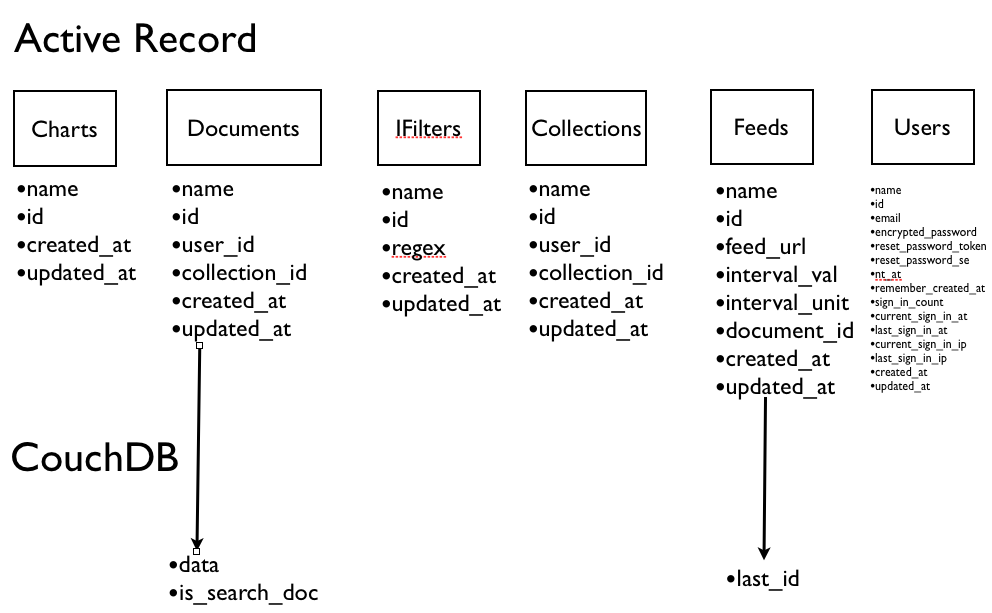
\includegraphics[width=120mm]{images/hatch_db_hybrid}
	\caption{The Hatch relational - non-relational database hybrid} 
	\label{hatch_db_hybrid}
	\end{center}
\end{figure}

The result is a relation - non-relational database hybrid. Hatch uses traditional 
relational database columns when the columns are ubiquitous, and can add columns to
a database entity (called scaffold) on the fly using CouchDB. For example, we create
a scaffold called Documents. Document always have a name, id, and collection/folder
they belong to. But, documents may have a data section, or they may not. That
data section may have infinite columns and rows of data, that would match the flat 
file they came from (like an Excel file). Or document may have any other data that
can be stored in JSON format. It is up to the Hatch interface, not database, to 
decide. And by allowing the interface to decide the structure and fields of data, Hatch
is by extension allowing the user to decide how to format data.

\pagebreak

\begin{figure}[h]
	\begin{center}
	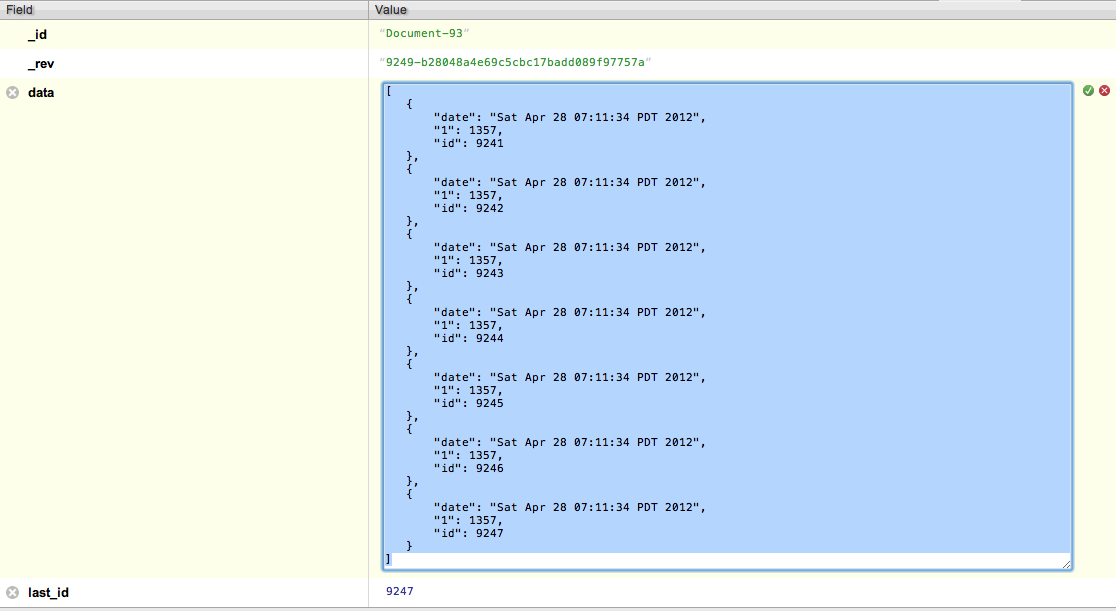
\includegraphics[width=120mm]{images/couchdb_json_ex}
	\caption{Typical representation of document data in CouchDB / JSON} 
	\label{couchdb_json_ex}
	\end{center}
\end{figure}

Most Rails applications that use CouchDB completely replace Active Record with some
library's version of it, like \textbf{couchrest's Active Model}. But if you replace
Active Record, you lose tons of support for libraries that lots of Rails developers
make, like pagination. 

Hatch gets around this by using its database hybrid, using a Ruby library called
\textbf{stuffing}. Stuffing is a link that ties Rails Active Record records with
CouchDB documents. It allows for rapid prototyping in development, and is a nice, modest
alternative to ripping out the guts of Active Record. Since the base model for 
database scaffolds are still Active Record, the huge amount of Rails Active Record based
libraries still work.



%\subsection{Search}
After the EcoData team addressed the issues with storing semi-structured data, the next 
big problem to address was how to efficiently search through the data. The interface 
that was desired was one much like Google's search; a simple search box, with two
buttons. The interface needs to be extremely simple yet powerful for it to be 
effective for non-technical users. 

\begin{figure}[h]
	\begin{center}
	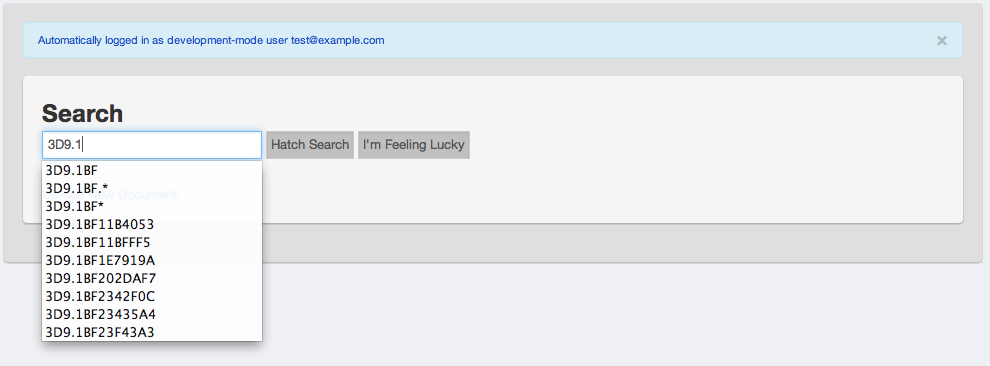
\includegraphics[width=120mm]{images/search_ss1}
	\caption{The search interface} 
	\label{search_ss1}
	\end{center}
\end{figure}

For example, when a user entered in a search like `3D9.1', it would be assumed that 
any data starting with `3D9.1' should be returned. Because Hatch assumes that
the user would want any data in the same row as the matching data, it returns
the entire row. 

For search, this could lead to a huge number of string comparisons in order to find
all values that match. This would make search impractically slow. Luckily, CouchDB allows
us to implement a practical solution to this problem.

\subsubsection{Views}
CouchDB uses precompiled queries called views. Views take developer-defined
query templates and apply them to every document that is created or updated in the 
database when the document is saved. The results are precompiled lookup tables 
(actually heaps/binary trees), which make searches fast. 

Hatch basically creates a view like the following pseudocode:
\singlespacing
\begin{lstlisting}
	for each document
		for each row
			for each column value in row
				emit(value, row)
\end{lstlisting}
\doublespacing

\texttt{emit()} is a function that tells CouchDB how to create the search B-Tree. It 
takes two arguments; the key that the tree node will take, and the value that the 
node will return if the key matches the search. Hatch says `every column value in a 
document is a key, and the return value is the data row it belongs to,' so if a search
matches a document value, the search results return the entire data row.

CouchDB makes Hatch's job easier by having internal methods for string matching. For
example, if a search for `3D9.1' is used with CouchDB startkey, CouchDB will return
any string starting with `3D9.1'. Hatch doesn't have to invent a query language to 
tell the database lots of parameters for matching values, which means users do not
need to learn a new query language either.

\begin{figure}[h]
	\begin{center}
	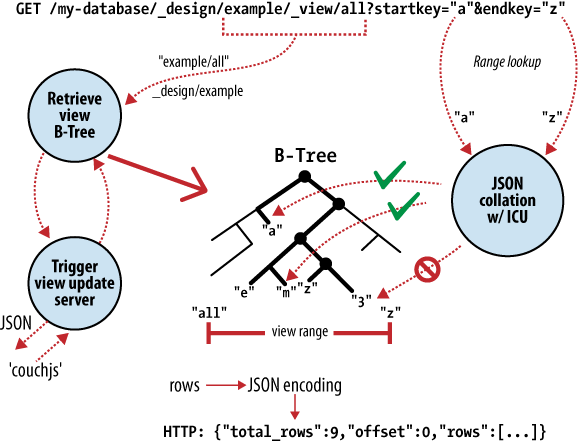
\includegraphics[width=120mm]{images/couchdb_b_tree}
	\caption{CoucbDB search through its internal binary tree.} 
	\label{couchdb_b_tree}
	\end{center}
\end{figure}

The other advantage to CouchDB is that it stores values in the B-Tree structure. For
string data types, this means that the database searches only within the `3D9.1' string range
in the tree. When the search sees a child node starting with `3D9.0', it instead picks
the child node staring with `3D9.1', and the entire `3D9.0' group is never searched 
through, which makes searches complete in a short time frame. 

%\subsection{Visualization}

When users are searching their data, it is important to get rapid feedback on the meaning,
shape, and size of the data they have found.  An intuitive method for this is through
charts, graphs, and other visualizations.

Hatch's visualizations allow users to accomplish these tasks. They allow users
to see unique data and graph values in comparison with other values. The Hatch
Documents interface allow users to do things like categorize data and then use
visualizations to graph the results.

\begin{figure}[h]
	\begin{center}
	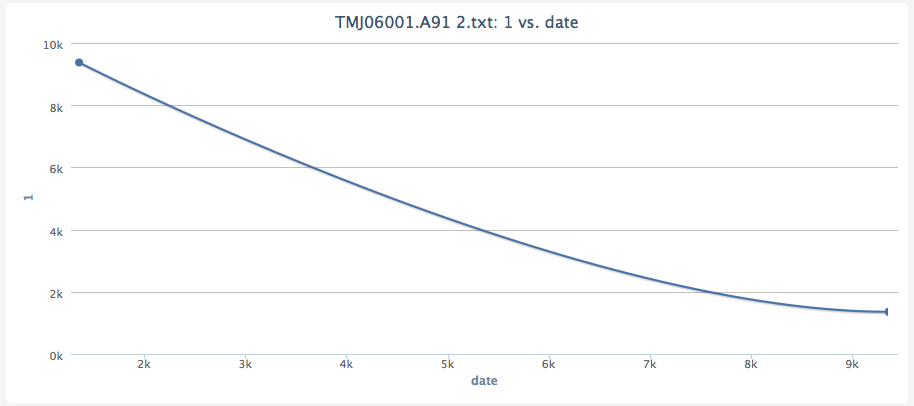
\includegraphics[width=120mm]{images/viz_ex1}
	\caption{A visualization example.} 
	\label{viz_ex1}
	\end{center}
\end{figure}

Hatch uses HighCharts, a JavaScript library, to perform visualizations. It
allows Hatch to incrementally stream new graph data to the client, instead of
resending all the graph data. This is useful when users are working on low
bandwidth connections, or with large datasets. By reducing unneeded data 
transfer, Hatch is able to work with larger datasets faster.

Hatch is able to check incrementally for new data. When data is graphed, it points towards the 
data in the document that needs visualization. If the data in the document changes,
the graph adds the data points to the graph without refreshing the page.

This opens up the possibility of Feeds. Feeds are scheduled events in Hatch that pull
JSON data from somewhere on the web. They push the data in to the document they point
to. This data can simultaneously be used by a visualization in order to immediately graph
the new data, as soon as a change is detected in the document.
The result is Live Charts, and documents that sync with data on the web when new data is 
available. Instead of doing a bulky request for data all at once, data can be taken
in smaller requests, and Hatch can give users a real-time view their data as it comes
into the system

%\section{Future Work}

Hatch has been specifically designed to be extensible and modular.  Because the needs
of the customer are so wide-ranging and would require a larger effort than our small
development team could reasonably complete in this time frame, Hatch has been
constructed with future extension in mind since day one.

Several major areas exist which could readily be improved or extended.  Included are
a few of these areas along with brief descriptions and time estimates, based on a team of
two working about 15 hours per week each.  Many other parts of Hatch could be extended,
but these are some of the most important areas for scientific research.

\subsection{New visualization types}
Currently, Hatch only fully supports single-series spline, line, and scatterplot
charts. Most of the code exists to extend this to categorical types and the
corresponding charts, such as pie and bar charts.  In addition, supporting
multiple-series data on a single chart is another obvious way to improve Hatch.

\textbf{Time estimate:} 1 week per chart type; 2 weeks for multiple-series data

\subsection{New data manipulation methods}
Hatch supports basic data manipulations such as filtering, sorting, and bringing
together columns from different data sets.  Obvious and useful extensions include
single-step joins between different data sets, log transforms, summary columns,
and suggested data joins.  These would form the basis for a more sophisticated
data manipulation pipeline that could be separated into a distinct package,
if desired.

\textbf{Time estimate:} 2 weeks per manipulation

\subsection{Performance enhancements}
Some areas of Hatch are not as responsive as could be.  While performance is not
crippling to the software, it can occasionally take a few seconds to complete
an action such as a search.  Some of this can be solved through more powerful
hardware (most tests were run on aging laptops), but algorithmic improvements
as well as general optimization could improve responsiveness greatly.

\textbf{Time estimate:} 1 month to double performance (more if other features are added)

\subsection{Cross-instance replication and sharing}
The original vision for Hatch included a system where each researcher could
run a localized Hatch instance and use the fully functional software on their
own machine.  Later, this data could be shared with a centralized Hatch instance,
or shared with other researcher's Hatch instances.  This requires solutions for
several difficult but solvable problems, and would require extensive testing.

\textbf{Time estimate:} 5 months

\section{Conclusion}
The Hatch project attempted to solve several difficult problems in an easy-to-use
package.  Due to time and resource constraints, Hatch must be seen as the beginning
of a comprehensive data management system that Hatch is positioned to grow into over time
through future efforts.

The developers followed accepted design patterns and consciously constructed the
software to be easily extended in every area.  Since it is likely this software
will be developed further in the future, a considerable amount of effort was spent
ensuring that each piece could be replaced or extended as necessary. Although the
project does not meet every need the customer has, it accomplished the goal of 
either meeting crucial needs or putting most of the pieces in place to allow the
straightforward extension of Hatch to meet them in the future.

Hatch defines a new model for aggregating, storing, and searching data. It embraces
RESTful design and the Don't Repeat Yourself mantra.
Hatch decouples design from data at all times;
something that is not too common in scientific research. As a result, the features
that are added to Hatch will continue to support any kind of data, as long as that 
data follows the core assumption Hatch makes: that data is in rows and columns.
Hatch embraces JSON as much as possible, providing JSON views whenever possible.
Feeds sync with JSON data on the web, and stores data in CouchDB's
native JSON format. The result is embracing open data exchange through the web in
one of the most ubiquitous and universal formats.

Although the certain features are not yet implemented, the essential core has
been demonstrated to work as desired, and the future functionality of Hatch is
only limited by developers and ideas.


%%%%%%%%% REFERENCES -- no limit

% this should include only items referenced in the project description
% it is not a bibliography of related reading.

% Each reference must include the names of all authors (in the same
% sequence in which they appear in the publication), the article and 
% journal title, book title, volume number, page numbers, and year of 
% publication. If the document is available electronically, the website 
% address also should be identified

\begin{thebibliography}{99}
\bibitem{gordon_moore} Manek Dubash (2005-04-13). "Moore's Law is dead, says 
	Gordon Moore". {\em Techworld}. Retrieved 2006-06-24
\bibitem{foster} Foster, James. {\em Visualizing Human Microbiome
        Ecosystems}. University of Idaho: Computer Science Colloquium, 
        December 7th 2010. Seminar.	

%\bibitem{new_life} Kanellos, Michael (19 April 2005). {\em New Life for 
%Moore's Law}. cnet. Retrieved 2009-03-19

\end{thebibliography}

%\printglossaries



\end{document}
